\documentclass[journal]{IEEEtran}
\usepackage{graphicx}
\usepackage[scriptsize]{caption}
\renewcommand{\arraystretch}{1.1}

\begin{document}

\newcommand{\labtitlegen}{
    \twocolumn[{
    \begin{center}
        \LARGE\labtitle \\ \bigskip \large\name \\ \bigskip
        \labsection \\ 
        \textbf{TA} \\ \taname \\% \bigskip \textbf{Lab Partners} \\
%        \partnername
    \end{center}
    }]
}

%% Change these variables
\newcommand{\labtitle}{Experiment 6: Diffraction Patterns}
\newcommand{\name}{604-296-523}
\newcommand{\labsection}{Section 2, Wednesday 8AM}
\newcommand{\labdate}{February 18, 2015}
\newcommand{\taname}{Elwin Martin}
\newcommand{\partnername}{Kari Kawashima}


%% This creates your lab cover page.
\labtitlegen

\newcommand{\mval}[3]{$#1 \pm #2 #3$}

\section{Introduction}

We will verify the diffraction patterns of pairs of vertical slits, by
measuring relative light itensity in the diffraction patterns of several pairs
of slits. A single known double-slit will be used to verify that the method
works, and the other three will have unknown dimensions.

In addition, the patterns created by a diffraction grating will be observed,
for both monochromatic red and white light, as will the diffraction pattern of
    the laser through a 2-dimensional grid. Both produce variations of the
    standard double-slit pattern, and allow similar measurements of the
    underlying diffraction structure (slit size or separation).

\section{Results}

\subsection{Double-Slit}

We set up the laser ($\lambda = 670$nm) and detector on either en of a
horizontal ruled track. The slits were placed between them, at a distance of
$41.6 \pm .05$ cm. An aperture, consisting of a single wide slit, was placed
directly in front of the detector.

The detector itself is a small track, perpendicular to the larger one, with a
total range of 5 cm. It contains a potentiometer, being driven by a 5V source.
This allows it to output a voltage correspondingly exactly to the distance
along the track. On top of the movable platform it has the end of a fiber-optic
cable, connected to a photometer which outputs a voltage proportional to the
intensity of light.

\begin{figure}[ht!]
\centering
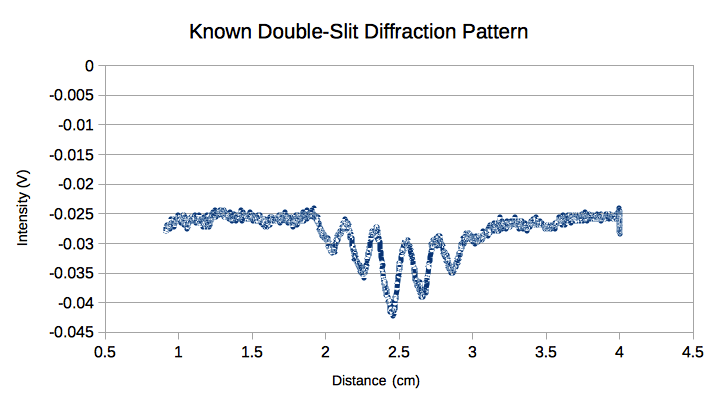
\includegraphics[width=80mm]{known.png}
\caption{Intensity amplitude pattern of known-dimension double slits.}
\label{known}
\end{figure}

%Single slit diffraction?

First, a double-slit of known dimensions (width 0.02 mm, separation 0.125 mm)
was used. It produced the intensity distribution in Figure~\ref{known}.

Three more double-slits, with unknown dimensions, were subsequently placed in
the same position as the first. Their intensity distributions are shown in
Figure ~\ref{unknown}. The exact intensity values have been modified by a
constant value so they fit in the graph - this does not change the analysis,
since the intensity values were already being measured relative to a non-zero
base intensity.

\begin{figure}[ht!]
\centering
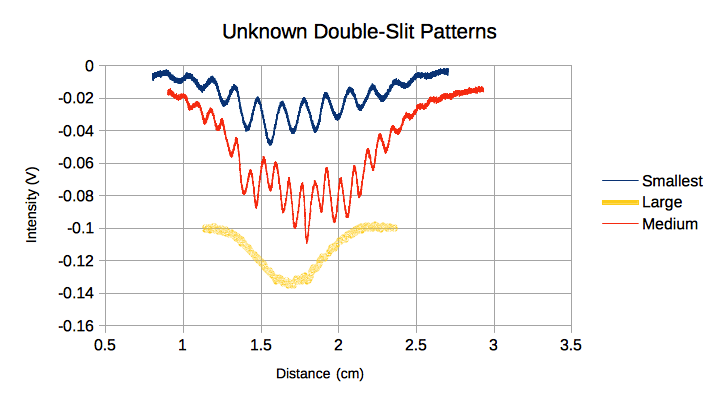
\includegraphics[width=80mm]{unknown.png}
\caption{Intensity amplitude pattern of the remaning three unknown-dimension
double slits.}
\label{unknown}
\end{figure}

Data for both measurements was collected at intervals of 0.01 s.

\subsection{Diffraction Grating}

A grating with 600 lines/mm we placed before the laser, with a beam expander
between them creating a vertical sheet of light from the laser's beam. The
result was several thin, vertical sheets of light spreading from the entry
point of the light into the diffraction grating. This is shown in
Figure~\ref{laser_grating}. The protractor was used to measure the angle
between maxima - in this case, the angle between the central beam and its two
adjacent maxima was 0.401 $\pm$ .02 rad. 

\begin{figure}[ht!]
\centering
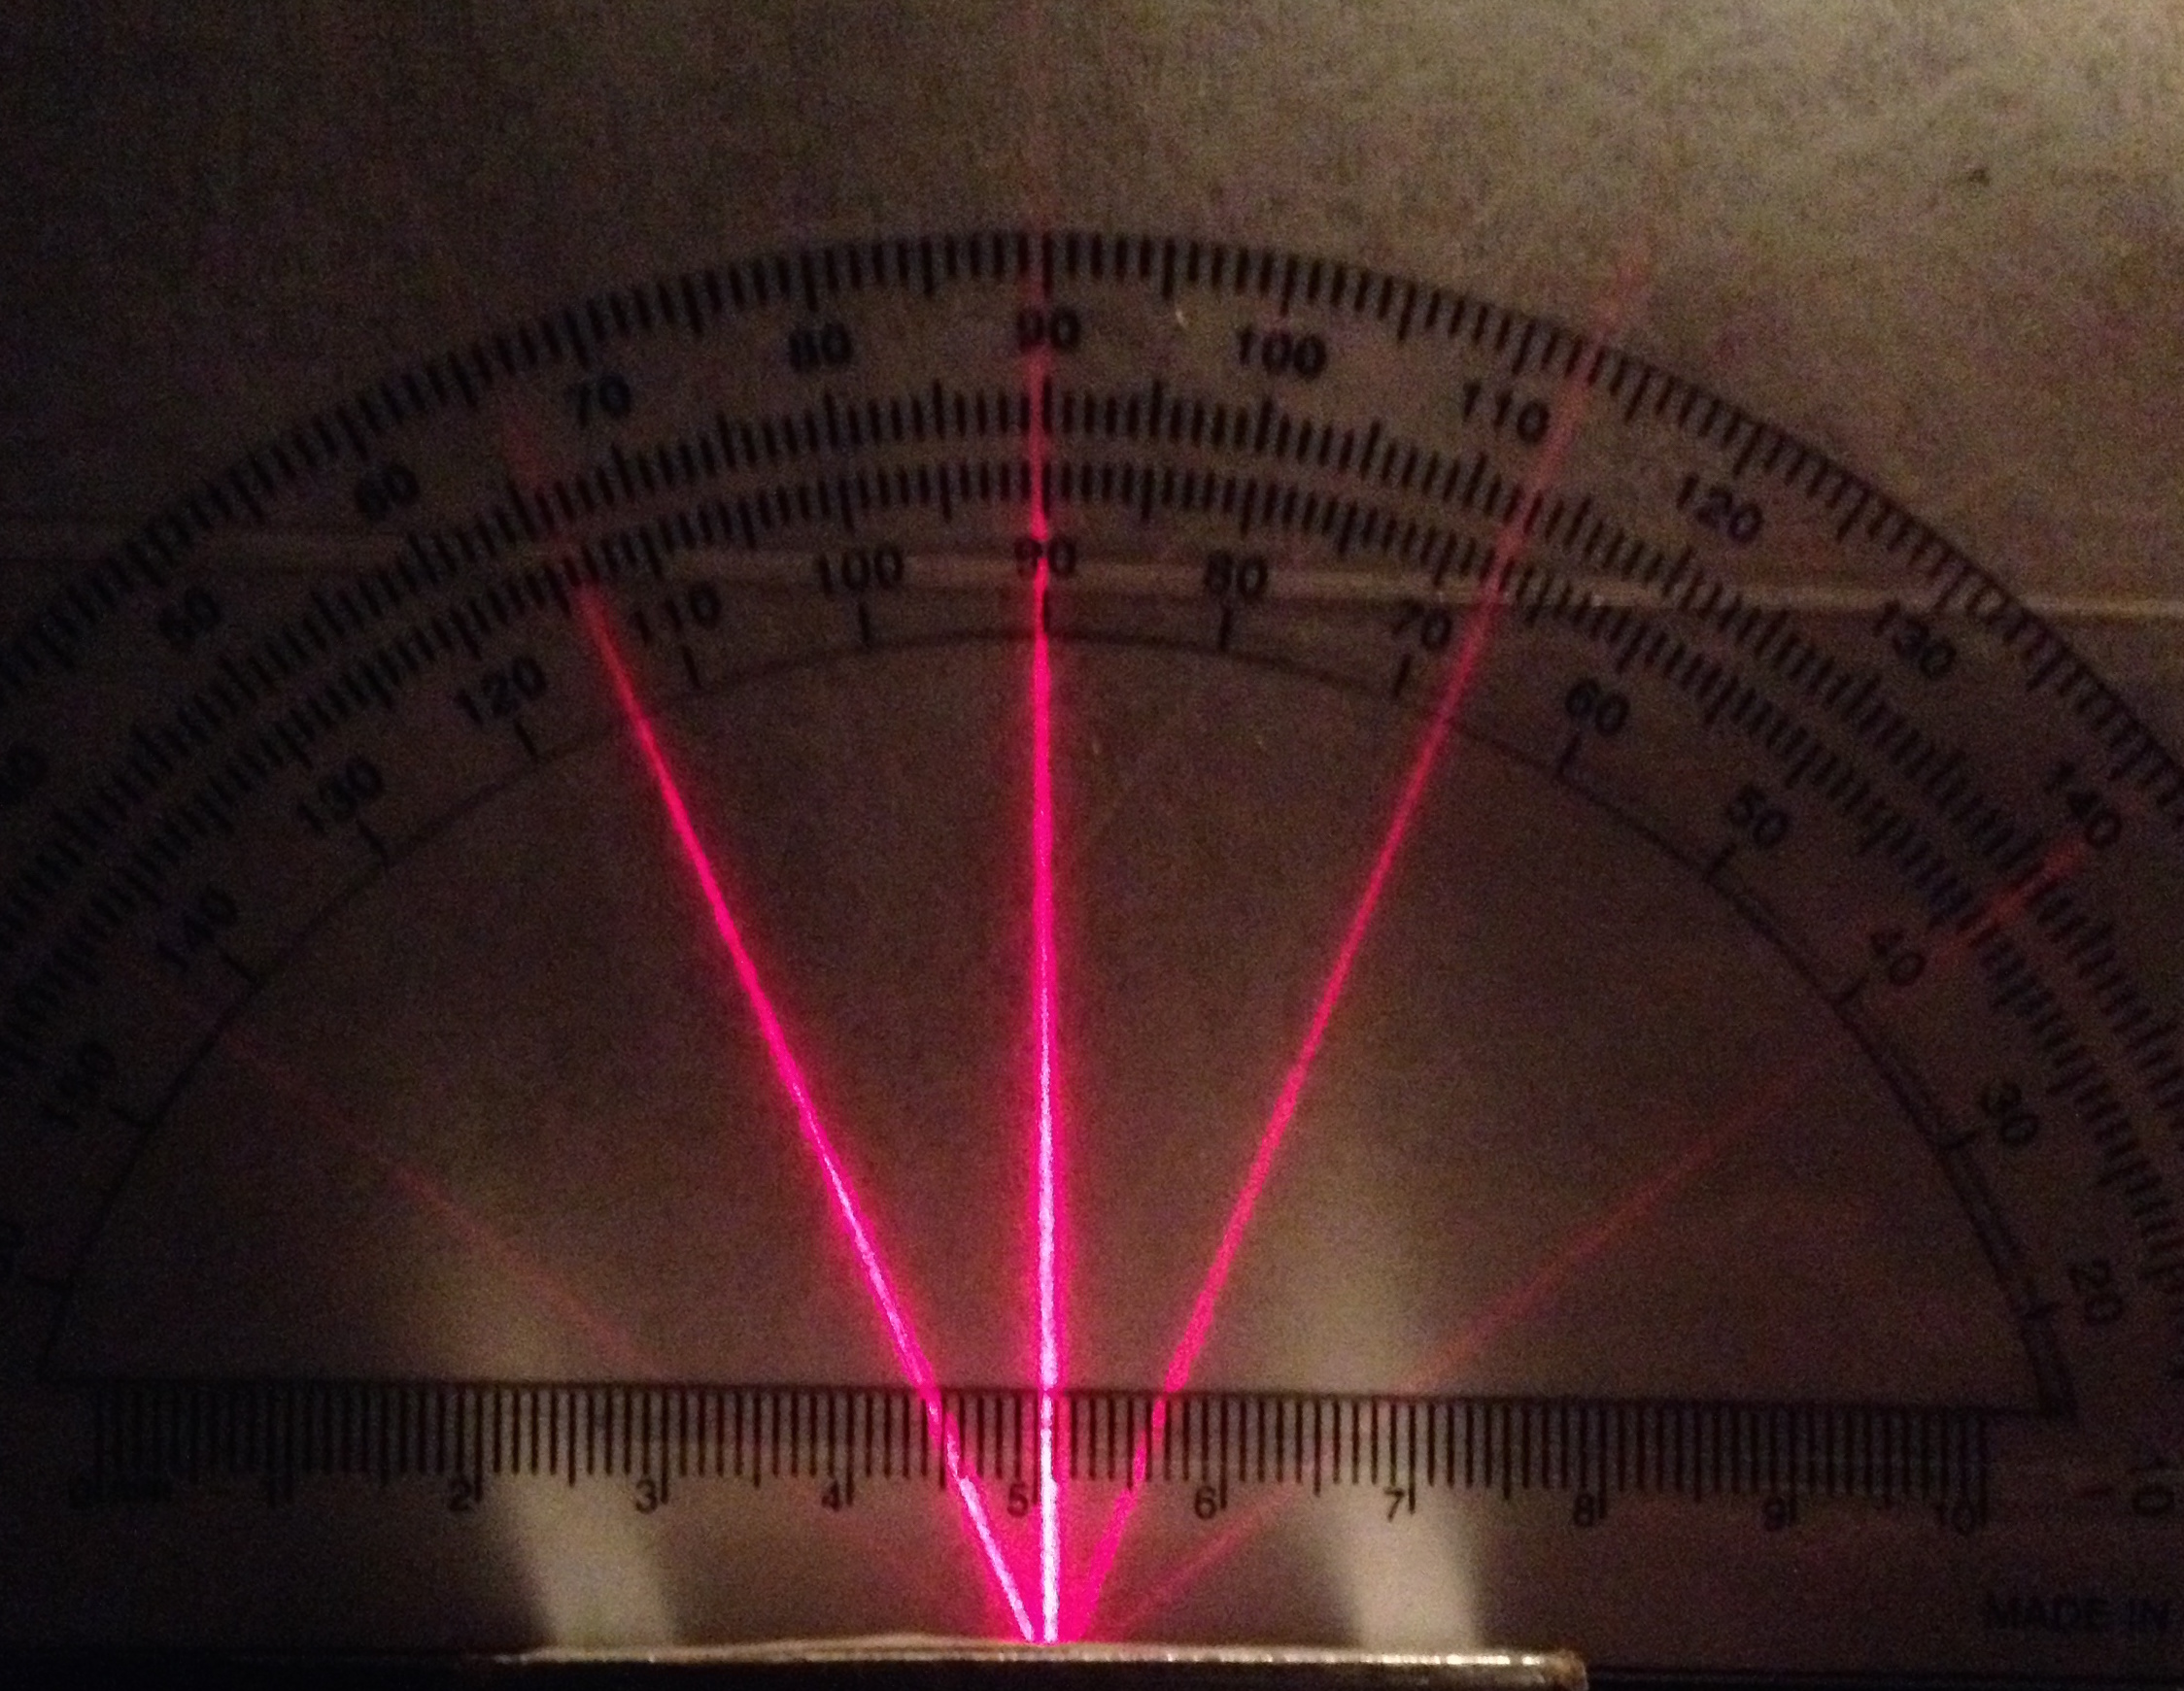
\includegraphics[width=60mm]{laser_grating.png}
\caption{Intensity amplitude pattern of the remaning three unknown-dimension
double slits.}
\label{laser_grating}
\end{figure}

The same process was used to measure differences in diffraction angles of
various wavelengths, by passing a vertical sheet of white light through the
same diffraction grating. In this case, the angle between the central beam and
the red beams were 0.39 $\pm$ .02 rad, the angle to the green beams were 0.34
$\pm$ 0.02 rad, and the angles to the blue beams were 0.28 $\pm$ .02 rad.

\subsection{Two-Dimensional Grid}

Whereas earlier a one-dimensional grating was used, now a two-dimmensional grid
pattern will be used to create a diffraction pattern. We used a similar setup
to the double-slit portion of this experiment, except instead of a detector we
used a piece of paper and a ruler to measure the dimensions of the diffraction
pattern. They were held the same distance from the grid (41.6 $\pm$ .05 cm).

The result was a spacing of 0.630 $\pm$ .003 cm per grid square. The pattern
was identical horizontally and vertically, making up a grid of nodes. In
addition, there was a secondary pattern of nulls - holes in the regular grid
pattern where nodes would have been. The first ones were 1.35 $\pm$ .05 cm from
the center of the pattern.

\section{Analysis}

The known double slit values - 0.02mm and .125mm - should match the values
extrapolated from the diffraction pattern. The latter values were obtained by
curve fitting Equation~\ref{double}, after giving reasonable starting values
estimated by eye from Figures \ref{known} and \ref{unknown}.

\begin{equation}
\label{double}
I(\theta, b, d, A) = A cos^2 \left[ \frac{2 \pi}{\lambda} d cos \theta
\right] \left[ \frac{sin (\pi b sin \theta / \lambda)}{\pi b \theta / \lambda}
\right]
\end{equation}


The known slit width returns values of d = .172 $\pm$ .007 mm and b = .018
$\pm$ .002 mm. These values have large uncertainties, obtained from the
diagonal of the covariance matrix. They were partly estimated from the errors given for each measured intensity, which were put at 5\% of the total intensity - this may be an overestimate, but it it 

The smallest slit has values of b = .0222 $\pm$ .0008 mm and d = .189 $\pm$
.007 mm. The middle slit has values of b = .0194 $\pm$ .0008 mm and d = .310
$\pm$ .006 mm. The largest slit could not be estimated, as there was too much noise.

The maxima conditions for a diffraction grating are the same as those for a
double-slit. Hence, the angle to the first maxima from the center is expected
to be

\begin{displaymath}
\theta = sin^{-1} \left( \frac{\lambda}{d} \right)
\end{displaymath}

Where d is the inverse of the lines per unit length. In this case, that angle
is expected to be 0.414 radians, to an unknown uncertainty (the grating and
wavelength values were specified without uncertainty). This differs from the
measured value of 0.401 $\pm$ .02 rad by -3.4\%.

For the multi-wavelength diffraction grating measurements, it will be assumed
that the wavelength of red light was 700 nm, the green light was 510 nm, and
the blue light was indigo at 430 nm. Using these values, Table 1 shows the
predicted and measured values for each color, and their percent error.

\begin{table}[ht]
\centering
\caption{\normalsize{Diffraction Grating Angles}}
\scalebox{.9}{
\begin{tabular}{|l|l|l|}
	\hline
	Color & Angle (rad) & Wavelength (nm)\\ \hline
	Red & .39 $\pm$ .02 & 630 $\pm$ 30 \\ \hline
	Green & .34 $\pm$ .02 & 550 $\pm$ 30 \\ \hline
	Blue & .28 $\pm$ .02 & 460 $\pm$ 30 \\ \hline
	\end{tabular}
}
\medskip
\caption{Table 1: Multi-wavelength diffraction grating angles.}
\end{table}

These wavelengths match roughly the colors observed and used to find the maxima
angles. More precise measurements would be needed for a more accurate
relationships

The grid pattern allows for very direct measurement of both the wire width and
separation, based on the locations of the double-slit nodes and single-slit
antinodes. The double slit nodes are located .630 $\pm$ .003 cm apart from each
other, and the grid was located 41.6 cm away, meaning the wires are .0442 $\pm$
.0003 mm apart. The distance of the antinodes from the center was 1.35 $\pm$
.05 cm, meaning the width of the wires was .021 $\pm$ .001 mm.

\section{Conclusion}

The values found for the slit width and separation are all suspect - the data
had several factors in it that could have prevented proper measurement. A large
amount of noise, and visible sinusoids beside the two that were supposed to be
present could have prevented a proper fit. The fits found did not visually
match the graph very well. This is seen in the error in the known slit
measurement - the measured value of .174 $\pm$ .007 mm is off by 37\%.

The diffraction grating results are much more accurate - though the angles were
measured by hand with a protractor, the laser result differs by only -3.4\%,
and the colored light result has wavelengths that fall near the centers of each
observed color.

The grid diffraction result, though no accepted values were given, appears to
be accurate - the pattern had very precise points, making measurements to
within the uncertainty of the ruler possible.

\end{document}


